\section{Metaheuristics}
\label{sec:metaheuristics}

In the following subsections is described the code implemented to solve the problem using
heuristics and metaheuristics, that is, the description of the code that actually implements
the heuristic framework, and the different heuristics used applied in the Local Search, GRASP
and BRKGA metaheuristics.

\subsection{Code}
\label{sec:metaheuristics:code}

In order to be able to implement, apply and compare different heuristics, random constructors
and chromosome decoders easily, an abstract class named \textit{problem} was implemented and
given a series of virtual methods. These methods will be implemented in subclasses and
each of them has a particular purpose: solve the problem using local search only, with or
without a random constructor or using genetic algorithms, .... This class will be used by the
other classes that implement the different metaheuristic algorithms, described in subsection
\ref{sec:metaheuristics:code:framework}, and has no attributes.

\subsubsection{Random number generator}
\label{sec:metaheuristics:code:rng}

Since part of this project requires randomly generated values for the GRASP and the BRKGA
metaheuristics, a simple interface was designed to test different random number generators.
This interface is the abstract class \textit{random\_generator}.

\hfill

This is implemented using the C++ 11's <random> header. It is a template that takes two
parameters: the random engine, and the type of the numbers to be generated. This is
a virtual class from which two other classes inherit its public and protected members.
These two classes are specialised for generating discrete random values and continuous
random values respectively.

\subsubsection{The \textit{problem} abstract class}
\label{sec:metaheuristics:code:problem}

The different functions that make up the \textit{problem} class can be classified into the
following categories.

\paragraph{Constructing a solution} \ 

\begin{lstlisting}
// Constructs an empty solution.
virtual problem *empty() const = 0;

// Constructs a solution from scratch. It uses a greedy algorithm.
// Returns the evaluation of the solution.
virtual double greedy_construct()
    throw(infeasible_exception) = 0;

// Explores this solution's neighbourhood and stores:
// - the best neighbour if BI is true (best improvement)
// - the first best neighbour if BI is false (first improvement)
// Best means a neighbour that maximizes the evaluate() function.
virtual void best_neighbour(pair<problem *, double>& best_neighbour,
    const local_search_policy& p = Best_Improvement) = 0;

// Constructs a randomized solution using a restricted candidate
// list (RCL) sorted using the parameter alpha.
// Returns the evaluation of the solution.
virtual double random_construct(random_number_generator *rng, double alpha)
    throw(infeasible_exception) = 0;

// Constructs a solution from a given chromosome.
// Returns the evaluation of the solution.
virtual double decode(const chromosome& c)
    throw(infeasible_exception) = 0;
\end{lstlisting}

\paragraph{Evaluating a solution} \

\begin{lstlisting}
// Evaluates the instance of this problem returning a scalar value
// representing its cost.
virtual double evaluate() const = 0;
\end{lstlisting}

\paragraph{Debugging a solution} \

\begin{lstlisting}
// Writes into the output stream the instance of this problem.
virtual void print(const string& tab = "", ostream& os = cout) const = 0;

// Checks all constraints regarding solution feasibility. Returns
// true if the solution is feasible. Returns false otherwise.
virtual bool sanity_check(const string& tab = "", ostream& os = cerr) const = 0;
\end{lstlisting}

\paragraph{Memory handling functions} \

\begin{lstlisting}
// Creates a copy of the instance of this problem.
virtual problem *clone() const = 0;

// Creates a copy of the instance of the problem passed as parameter.
virtual void copy(const problem *p) = 0;

// Clears the memory used by the instance of this problem.
// Everything is reset so that the method construct would create
// a solution to the problem if it were to be called.
virtual void clear() = 0;
\end{lstlisting}

More details can be found in the documentation.

\subsubsection{Metaheuristics framework}
\label{sec:metaheuristics:code:framework}

The metaheuristics framework has been implemented in C++. A simple UML diagram describing the
inheritance relationships between classes can be seen in figure \ref{fig:metaheuristics-UML}.
This framework was implemented this way so as to allow more flexibility in future projects.
Each class uses the \textit{problem} abstract class to model as generally as possible the
different algorithms.

\begin{figure}[H]
    \centering
    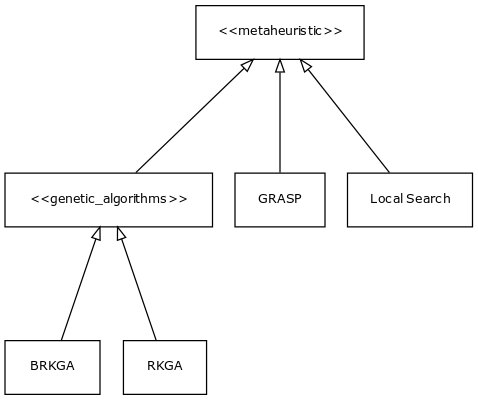
\includegraphics[scale=0.5]{metaheuristics-framework}
    \caption{Simplified UML diagram describing the metaheuristics framework.}
    \label{fig:metaheuristics-UML}
\end{figure}

\subsection{Preliminaries}
\label{sec:metaheuristics:preliminaries}

In this section are described few notations and concepts for the sake of understandability of
this text:

\begin{itemize}
    \item Sets of cities served by location $\iloc$: $P_\iloc$ and $S_\iloc$. These two sets
    are defined in section \ref{sec:ILP-form:constraints}, when defining the constraint
    \ref{cstr:centre-not-overbooked} and represent the cities served by $\iloc$ with a
    primary and a secondary role respectively.
    
    \item Occupied capacity of a location: $K(\iloc)$: this can be formally defined using the
    usual formula:
    \begin{equation}
    K(\iloc) = \sum_{\icity \in P_\iloc} p_c + 0.10 \cdot \sum_{\icity \in S_\iloc} p_c
    \end{equation}
    
    \item Added capacity of a city $\icity$ to a location $\iloc$ with a role $r$:
    $K_a(\icity, r)$. This measures the increment of the capacity in location $\iloc$
    ($K(\iloc)$) when making location $\iloc$ serve city $\icity$ with a role $r$. This is
    formally defined as follows:
    \begin{equation}
    K_a(\icity, r) =
        \left \{
        \begin{array}{l l}
            p_\icity,            & r= \text{ primary} \\
            0.10 \cdot p_\icity, & r= \text{ secondary}
        \end{array}
        \right.
    \end{equation}
    
    Therefore:
    \[
    K(\iloc) =  \sum_{\icity \in P_l} (K_a(\icity, primary) +
                \sum_{\icity \in S_l} K_a(\icity, secondary)
    \]
    
    \item Capacity gap in a location $\iloc$ with a centre installed when assigning a city
    $\icity$ with a role $r$: $G$. This simply measures how much capacity is left in location
    $\iloc$ after it has been assigned to city $\icity$ with role $r$, and can only be
    measured if that     location has a centre $\icentre$ installed. $G$ is formally defined
    as follows:
    \begin{equation}
    G(\iloc, \icity, \icentre, r) = c_\icentre - (K(\iloc) + K_a(\icity, r))
    \end{equation}
    
    Notice that for the assignation of $\iloc$ to $\icity$ with role $r$ to be valid, $G$
    must be equal or greater than 0 ($G(\iloc, \icity, \icentre, r) \ge 0$).
    
\end{itemize}

Remember that $p_\icity$ denotes the population of city $\icity$.

\subsection{Greedy algorithms}
\label{sec:metaheuristics:greedy-algorithms}

In this section are described the different heuristics implemented to solve the problem using
Local Search. This includes the greedy construction algorithm and the neighbourhood
exploration algorithm.

\subsubsection{Greedy construction algorithm}
\label{sec:metaheuristics:greedy-algorithms:greedy-constructor}

The greedy construction algorithm follows this basic procedure: while there are still cities
lacking a primary or a secondary location, consider all possible candidates for assignation
and take the one that minimises the cost of the greedy function. When the candidate that
minimises this cost is found what remains is to add it to the solution being constructed.
This step will be repeated until there are no more candidates left. A candidate for this
algorithm is the tuple $<\icity, \iloc, r>$, where $\icity \in \city$ is a city,
$\iloc \in \loc$ is a location and $r$ represents represents the role that location $\iloc$
will have when serving city $\icity$ (that is either ``primary'' or ``secondary''). It is
worth being mentioned that we do not consider as valid candidates those that contain a
location that is not far enough from the other locations with a centre installed and neither
those with a location that is already serving the city in the candidate. Therefore, the
candidates are ``filtered'' using the distance criterion and checking already assigned roles.
Then they are evaluated using the usual capacity and distance (between city and location)
constraints. The greedy constructor algorithm is, therefore, as follows:

\hfill

\begin{algorithm}[H]
    \label{alg:greedy-construct}
    \DontPrintSemicolon
    
    \caption{Greedy construction}
    \KwIn{$Problem$ the specification of the problem}
    \KwOut{$S$ a possibly feasible solution to $Problem$}
    
    \SetKwProg{Fn}{Function}{ is}{end}
    \Fn{\textsc{GreedyConstruct}$(Problem)$} {
        $S := \varnothing$ empty solution \;
        $U := \varnothing$ the set of locations used \;
        $k := 1$, $K := 2|\city|$ the number of assignations to be made\;
        \While {$k \le K$} {
            $F := \varnothing$ the candidate list\;
            \For {$<\icity, \iloc> \; : \; \icity \in \city, \; \iloc \in \loc$} {
                $d := \text{min}
                    \{
                    d(\iloc, \iloc') \; : \;
                        \iloc' \in \loc \; \wedge \; 
                        \iloc' \neq \iloc \; \wedge \; 
                        \iloc' \text{ has a centre installed}
                    \}
                $\;
                \If
                {$\neg (\icity \in P_\iloc$ $\vee$ $\icity \in S_\iloc) \wedge d \ge D$}
                {
                    \lIf {$\icity \notin P_\iloc$} {
                        $F := F \cup \{<\icity, \iloc, primary>\}$
                    }
                    \lIf {$\icity \notin S_\iloc$} {
                        $F := F \cup \{<\icity, \iloc, secondary>\}$
                    }
                }
            }
            \lIf {$F = \varnothing$} {
                \Return Infeasible\label{alg:gc:return-infeasible}
            }
            $m := \textsc{MinCandidate}(F, \Box)$\;
            $S \leftarrow \textsc{Assign}(m_\icity, m_\iloc, m_r)$\;
            $U := U \cup \{ m_\iloc \}$, $k := k + 1$\;
        }
        $S\leftarrow\textsc{FindAndAssignCentres}$($U$)
            \label{alg:gc:find-and-assign-centres}\;
        \Return $S$\;
    }
\end{algorithm}

\hfill

The function in line \ref{alg:gc:find-and-assign-centres} simply loops over all locations
used $\iloc$ in $U$ and finds the cheapest centre that can serve the cities assigned to each
location. Even though the procedure is designed to terminate by returning infeasibility when
a candidate can not be found (line \ref{alg:gc:return-infeasible}), the existence of at least
one centre type available for all locations when line \ref{alg:gc:find-and-assign-centres} is
reached is not guaranteed.

\hfill

The symbol $\Box$ denotes any greedy function. Several greedy cost functions were defined:

\begin{equation}
f_1(<\icity, \iloc, r>) =
    \left \{
    \begin{array}{l l}
        d(\icity, \iloc),                   & \text{case 1} \\
        +\infty,                            & \text{case 2} \\
        d(\icity, \iloc) \cdot i_\icentre,  & \text{case 3} \\
        +\infty,                            & \text{otherwise}
    \end{array}
    \right.
\label{eq:greedy-cost-dist}
\end{equation}

\begin{equation}
f_2(<\icity, \iloc, r>) =
    \left \{
    \begin{array}{l l}
        K(\iloc) + K_a(\icity, r),                       & \text{case 1} \\
        +\infty,                                         & \text{case 2} \\
        (K(\iloc) + K_a(\icity, r)) \cdot i_\icentre,    & \text{case 3} \\
        +\infty,                                         & \text{otherwise}
    \end{array}
    \right.
\label{eq:greedy-cost-pop}
\end{equation}

\begin{equation}
f_3(<\icity, \iloc, r>) =
    \left \{
    \begin{array}{l l}
        K(\iloc) + K_a(\icity, r) + d(\icity, \iloc),    & \text{case 1} \\
        +\infty,                                         & \text{case 2} \\
        (K(\iloc) + K_a(\icity, r)) + d(\icity, \iloc) \cdot i_\icentre,
                                                         & \text{case 3} \\
        +\infty,                                         & \text{otherwise}
    \end{array}
    \right.
\label{eq:greedy-cost-dist-pop}
\end{equation}

Case 1 is found when location $\iloc$ is already serving some cities and can also serve city
$\icity$ with role $r$, case 2 is found when location $\iloc$ can not serve city $\icity$,
whether it is already serving other cities or not, and case 3 when location $\iloc$ is not
serving any other city and can serve city $\icity$ with centre $\icentre$ installed in it.
In case 3, centre $\icentre$ is the cheapest centre that can serve city $\icity$.
$d(\icity, \iloc)$ denotes the distance between city $\icity$ and location $\iloc$.
Obviously, each of these functions lead to different in terms of the solution's cost, but it
is only the last function (see greedy function \ref{eq:greedy-cost-dist-pop}) that makes this
algorithm behave the best: the other two functions made it impossible for the algorithm to
find centres available for some of the locations used (remember line
\ref{alg:gc:find-and-assign-centres}) whereas the last seems to guarantee that,
if the construction turns out to be infeasible, it is because no feasible candidate was
found. All experiments will be carried out using this function.

\subsubsection{Neighbourhood exploration}
\label{sec:metaheuristics:greedy-algorithms:neighbourhood-exploration}

Since we are dealing with a minimisation problem, a neighbour of a solution could be a very
similar instance but with a centre installed less, or with a cheaper centre. That is,
obtaining a new neighbour from a given solution consists on finding a location $\iloc \in
\loc$, with a centre installed, removing it if possible and reassigning the cities it served
to other locations with a centre installed. In case it is not possible to remove it, we will
try to replace it with a cheaper one. Notice that it would not make much sense to try
replacing a centre in the first place since removing it leads to a much better solution. And,
only when it can not be removed does it make sense to try and replace it. The pseudocode of
the algorithm is as follows:

\hfill

\begin{algorithm}[H]
    \label{alg:find-neighbour}
    \DontPrintSemicolon
    
    \caption{Finding a neighbour}
    \KwIn{$S$ feasible solution, $\iloc$ location with a centre installed}
    \KwOut{$B$ a feasible solution with a cost equal to or smaller than $S$'s}
    
    \SetKwProg{Fn}{Function}{ is}{end}
    \Fn{\textsc{FindNeighbour}$(S, \iloc)$} {
        $B$ :=  copy($S$)\;
        $\city_{\iloc} := $ cities served by $\iloc$\;
        $N$ := \textsc{CanRemoveCentre($\city_{\iloc}, \iloc$)}
            \label{alg:ne:remove-centre}\;
            
        \If {$N \neq \varnothing$} { \label{alg:ne:check-if-can-remove}
            \For {$\icity \in \city_{\iloc}$} {
                $B \leftarrow$ \textsc{Remove}($\icity, l$)
                    \label{alg:ne:remove-assignation}\;
                
                \lIf {$\icity \in P_{\iloc}$} {
                    $B \leftarrow$ \textsc{Assign}($\icity, N_{\icity}, primary$)
                        \label{alg:ne:new-assignation-1}
                }
                \lElseIf {$\icity \in S_{\iloc}$} {
                    $B \leftarrow$ \textsc{Assign}($\icity, N_{\icity}, secondary$)
                        \label{alg:ne:new-assignation-2}
                }
            }
        }
        \Else {
            $I_\iloc := $ installed centre in location $\iloc$\;
            $S := $ sort centres by installation cost\;
            \For {$\icentre \in S$} {
                \If {\textsc{CanServeCities}$(\icentre,P_\iloc,S_\iloc) \wedge
                    i_\icentre<i_{I_\iloc}$}
                {
                    $B \leftarrow$ \textsc{ReplaceCentre}($I_\iloc$, $\icentre$)
                        \label{alg:ne:replace-centre}\;
                    Break\;
                }
            }
        }
        \Return $B$
    }
\end{algorithm}

\hfill

We find in this algorithm some functions that need some clarification. To begin with, the
function we find in line \ref{alg:ne:remove-centre} (\textsc{CanRemoveCentre}) takes the
cities location $\iloc$ is serving along with the appropriate role $\city_\iloc$, and the
location $\iloc$ itself. With these two parameters, this function tries to assign each of
the cities in $\city_\iloc$ to other locations with a centre already installed. These
locations are then returned in a structure where, for each city, we find the new location
that will serve it. If no locations are returned (line \ref{alg:ne:check-if-can-remove})
then the algorithm wll try to replace the centre.

\hfill

The typical constraints of distance and capacity have to be satisfied in order to choose a
location for city $\icity$ but the location chosen is, among those that satisfy these
constraints, the closest in distance to the city and the one that maximises the capacity gap.
Therefore, the new assignations are done greedily: that is, they are done in increasing order
of added capacity.

\hfill

\begin{algorithm}[H]
    \label{alg:can-remove-centre}
    \DontPrintSemicolon
    
    \caption{Removing a centre}
    \KwIn{$\city_{\iloc}$ cities served by location $\iloc$, $\iloc$ the location with the
    centre we are trying to remove}
    \KwOut{$N$ a set of new locations that can serve the cities in $\city_{\iloc}$}
    
    \SetKwProg{Fn}{Function}{ is}{end}
    \Fn{\textsc{CanRemoveCentre}$(\city_\iloc, \iloc)$} {
        $N := \varnothing$\;
        $\Gamma_\iloc := $ sort cities in $\city_\iloc$ by added capacity $K_a$\;
        
        \For {$\icity \in \Gamma_\iloc$} {
            $Q := \varnothing$\;
            \For {$\iloc' \in \loc \; : \; \iloc'$ has a centre installed} {
                \lIf {location $\iloc'$ satisfies all constraints} {
                    $Q := Q \cup \{\iloc'\}$
                }
            }
            \If {$Q \neq \varnothing$} {
                $m_\iloc := \textsc{MinDistGap}$($Q$)\;
                $N := N \cup \{ < \icity, m_\iloc > \} $\;
            }
        }
        
        \Return $N$
    }
\end{algorithm}

\hfill

The functions \textsc{Remove}, \textsc{Assign} and \textsc{ReplaceCentre} found in lines
\ref{alg:ne:remove-assignation}, \ref{alg:ne:new-assignation-1} and
\ref{alg:ne:new-assignation-2}, and \ref{alg:ne:replace-centre} of algorithm
\ref{alg:find-neighbour} respectively, are quite self-explanatory. They make a location
stop serving a city, updating all data structures, assign a location to serve a city, also
updating all necessary data structures, and replacing one centre installed for another,
respectively.

\hfill

The actual neighbourhood exploration algorithm is as follows: given an initial solution, for
every pair of different locations with a centre installed in them - in the initial solution -
try to apply the procedure described above. The returned value is called a neighbour.
Depending on the policy of the exploration (either \textsc{First-Improvement} or
\textsc{Best-Improvement}) the procedure will stop when it finds the first neighbour with
lower cost than the initial solution or will explore all possible neighbours and will return
the one with lowest cost.

\hfill

\begin{algorithm}[H]
    \label{alg:neighbourhood-exploration}
    \DontPrintSemicolon
    \caption{Exploring the neighbourhood}
    \KwIn{$S$ feasible solution, $Policy$ the neighbourhood exploration policy}
    \KwOut{$B$ a feasible solution with a cost equal to or smaller than $S$}
    
    \SetKwProg{Fn}{Function}{ is}{end}
    \Fn{\textsc{NeighbourhoodExploration}$(S, Policy)$} {
        $B := copy(S)$\;
        \For {$\iloc \in \loc$} {
            $N := \textsc{FindNeighbour}(S, \iloc)$\;
            \If {$cost(N) < cost(B)$} {
                $B := N$\;
                \lIf {$Policy = \textsc{First-Improvement}$} {
                    \Return $B$
                }
            }
        }
        \Return $B$
    }
\end{algorithm}

\hfill

\subsection{GRASP - Randomised construction}
\label{sec:metaheuristics:randomised-construction}

In this section is described the random constructor that will be used by the GRASP
metaheuristic \cite{GRASP}. This constructor basically follows the same procedure in the greedy
constructor algorithm \ref{alg:greedy-construct}: it will construct the candidate list by
using the same definition of what a candidate is and using the greedy cost function
\ref{eq:greedy-cost-dist-pop}. Then, by using the parameter $\alpha$ it will construct the
Restricted Candidate List, choose one of the candidates at random and add it to the solution.
The following pseudocode models the usual procedure for doing this.

\hfill

\begin{algorithm}[H]
    \label{alg:random-constructor}
    \DontPrintSemicolon
    
    \caption{Randomised construction}
    \KwIn{$Problem$ the specification of the problem}
    \KwOut{$S$ a possibly feasible solution to $Problem$}
    
    \SetKwProg{Fn}{Function}{ is}{end}
    \Fn{\textsc{RandomConstructor}$(Problem)$} {
        $S := \varnothing$ empty solution \;
        $U := \varnothing$ the set of locations used\;
        $k := 1$\;
        $K := 2|\city|$ the number of assignations to be made\;
        \While {$k \le K$} {
            $F := $ Build candidate list as in algorithm \ref{alg:greedy-construct}
                with greedy function $\Box$\;
                
            \lIf {$F = \varnothing$} {
                \Return Infeasible
            }
            
            $s := \textsc{Min}(F, \Box)$\;
            $S := \textsc{Max}(F, \Box)$\;
            
            $RCL := \varnothing$ the Restricted Candidate List\;
            \For {$f \in F$} {
                \lIf {$\Box_f \le s + \alpha \cdot (S - s)$} {
                    $RCL := RCL \cup \{ f \}$
                }
            }
            
            $m := $ select one element in the RCL at random\;
            $S \leftarrow \textsc{Assign}(m_\icity, m_\iloc, m_r)$\;
            $U := U \cup \{ m_\iloc \}$\;
            $k := k + 1$\;
        }
        $S \leftarrow \textsc{FindAndAssignCentres}$($U$)\;
        \Return $S$\;
    }
\end{algorithm}

\hfill

Again, the symbol $\Box$ denotes any greedy function. The actual GRASP procedure is as
follows:

\hfill

\begin{algorithm}[H]
    \label{alg:grasp}
    \DontPrintSemicolon
    
    \caption{Greedy Randomised Search Procedure}
    \KwIn{$Problem$ the specification of the problem, $I \in \mathbb{N}$ a number of
    iterations, $Policy$ the policy of the local search procedure}
    \KwOut{$B$ a feasible solution to $Problem$}
    
    \SetKwProg{Fn}{Function}{ is}{end}
    \Fn{\textsc{GRASP}$(Problem, I, Policy)$} {
        $B := \varnothing$ empty solution\;
        $i := 1$\;
        \While {$i \le I$} {
            $R := $\textsc{RandomConstructor}($Problem$)\;
            $L := $\textsc{NeighbourhoodExploration}($R, Policy$)\;
            \lIf {$cost(L) < cost(B)$} {
                $B := L$
            }
            $i := i + 1$\;
        }
        \Return $B$\;
    }
\end{algorithm}

\hfill

We can consider that the cost of an empty solution is $+\infty$.

\subsection{BRKGA - Chromosome decoder}
\label{sec:metaheuristics:chromosome-decoder}

In this section is described a simple algorithm that will be used by the BRKGA procedure
\cite{brkga}. BRKGA stands for Biased Random-Key Genetic Algorithm and is a procedure that,
roughly, consists on finding the fittest individuals within a population and ``crossing'' them with
not-so-fit individuals of the same population to produce a great variety of individuals,
some of which are quite likely to be better than its parents, and, after repeating this
step several times, find the fittest individual. To do that, individuals are represented with
chromosomes, a set of genes, that need to be decoded into our solution in order to evaluate
their fitness. This decoder algorithm is described later in this section in algorithm
\ref{alg:chromosome-decoder}. The BRKGA procedure works as follows:

\hfill

\begin{algorithm}[H]
    \label{alg:brkga}
    \DontPrintSemicolon
    
    \caption{Biased Random-Key Genetic Algorithm}
    \KwIn{$Problem$ the specification of the problem, $G \in \mathbb{N}$ a number of
    generations, $s$ the size of each individual's chromosome, $p$ the size of the population,
    $p_e$ the size of the elite population, $p_m$ the size of the mutant population, $\rho_e$
    the inheritance probability}
    \KwOut{A feasible solution to $Problem$}
    
    \SetKwProg{Fn}{Function}{ is}{end}
    \Fn{\textsc{BRKGA}$(Problem, G, s, p, p_e, p_m, \rho_e)$} {
        $\mathcal{P} := $\textsc{InitializePopulation}($p$, $s$)
            \label{alg:brkga:initialize-pop}\;
            
        $\mathcal{E} := $\textsc{TrackEliteIndividuals}($\mathcal{P}, p_e$)
            \label{alg:brkga:initialize-elite}\;
        
        $g := 1$\;
        \While {$g \le G$} {
            $\mathcal{M} := $\textsc{MutantPopulation}($p_m$)
                \label{alg:brkga:gen-mutant}\;
                
            $\mathcal{R} := $\textsc{Crossover}($\mathcal{E}, P-\mathcal{E}, p - p_e - p_m,
            \rho_e$)
                \label{alg:brkga:gen-cross}\;
            
            $\mathcal{P} := \mathcal{E} \cup \mathcal{M} \cup \mathcal{R} $
                \label{alg:brkga:redefine}\;
                
            $\mathcal{E} := $\textsc{TrackEliteIndividuals}($\mathcal{P}$)
                \label{alg:brkga:keep-track}\;
            
            $g := g + 1$\;
        }
        \Return \textsc{FittestIndividual}($\mathcal{E}$)\;
    }
\end{algorithm}

\hfill

The procedure starts by initialising the population set, with a number $p$ of individuals,
each represented by a chromosome of size $s$, and tracks the $p_e$ fittest individuals
$\mathcal{E}$, (lines \ref{alg:brkga:initialize-pop} and \ref{alg:brkga:initialize-elite}).
Then, the procedure will proceed to produce the $G$ generations of individuals, one depending
on the previous one. A generation is produced by creating a set of $p_m$ random individuals
(the mutant set $\mathcal{M}$, line \ref{alg:brkga:gen-mutant}) and then cross some of them
with a randomly chosen individual from $\mathcal{E}$ to produce the crossover population
$\mathcal{R}$ (line \ref{alg:brkga:gen-cross}). The new population set is then defined as the
previous elite set of individuals, together with the mutant and the crossover populations
(line \ref{alg:brkga:redefine}). Since there are new individuals in this population, there may
be new elite individuals that need to be kept track of. That is were we redefine the set
$\mathcal{E}$, in line \ref{alg:brkga:keep-track}. Finally, the procedure returns the fittest
individual of the elite set, that is also the fittest individual of the whole population.

\hfill

The crossover is done by using the inheritance probability $\rho_e$: for $p - p_m - p_e$
non-elite individuals $u$, an elite individual $e$ is randomly chosen and then they are
crossed to create a new individual $z$. If $\sigma_u$, $\sigma_e$ and $\sigma_z$ are the
chromosomes of the individuals respectively, the $k$-th gene of the newly generated
individual, $\sigma_{z, k}$ is chosen between $\sigma_{u, k}$ and $\sigma_{e, k}$ according
to the aforementioned inheritance probability $\rho_e$: if a randomly generated scalar
$\phi \in [0, 1]$ is smaller than $\rho_e$ then $\sigma_{e, k}$ is chosen. If it is greater
then $\sigma_{u, k}$ is chosen instead.

\hfill

\begin{algorithm}[H]
    \label{alg:brkga:crossover}
    \DontPrintSemicolon
    
    \caption{Generating the crossover population}
    \KwIn{$\mathcal{E}$ elite set of individuals, $\mathcal{F}$ non-elite set of individuals,
    $p_c$ number of crossover individuals, $\rho_e$ probability of inheritance}
    \KwOut{$\mathcal{R}$ set of crossover individuals}
    
    \SetKwProg{Fn}{Function}{ is}{end}
    \Fn{\textsc{BRKGA}$(\mathcal{E}, \mathcal{F}, p_c, \rho_e)$} {
        $\mathcal{R} := \varnothing$\;
        $r := 1$\;
        \While {$r \le p_c$} {
            $e := $\textsc{RandomChoice}($\mathcal{E}$)\;
            $u := $\textsc{RandomChoice}($\mathcal{F}$)\;
            $z := \varnothing$ new individual\;
            $k := 1$\;
            \While {$k \le |\sigma_x|$} {
                $\phi := $\textsc{Random}(0, 1)\;
                \lIf {$\phi \le \rho_e$} {
                    $\sigma_{z, k} := \sigma_{e, k}$
                }
                \lElse {
                    $\sigma_{z, k} := \sigma_{u, k}$
                }
                $k := k + 1$\;
            }
            $\mathcal{R} := \mathcal{R} \cup \{z\}$\;
        }
        \Return $\mathcal{R}$\;
    }
\end{algorithm}

\hfill

As it has been mentioned, finding the fittest individual relies on the fact that a chromosome
$\sigma$ has to be decoded into a feasible solution. The fitness of the individual is, then,
the cost of the solution. In this case, the chromosome decoder is also based on a previous
algorithm: the greedy constructor. This decoder will sort the chromosome so that the lowest
values of the genes are placed at the beginning and the highest at the end. This yields an
order of these chromosomes that will be used to construct a solution. The number of genes for
each chromosome is equal to the number of cities in the instance $|\city|$. The indexes that
represent the order of the genes in the chromosome are then interpreted as city indexes and
then, for each city, we find the best location candidate according to some greedy function and
assign it to the solution. Once all cities have been assigned a primary and a secondary
location, remains only to assign centres to the locations used.

\hfill

\begin{algorithm}[H]
    \label{alg:chromosome-decoder}
    \DontPrintSemicolon
    
    \caption{Randomised construction}
    \KwIn{$\sigma$ a chromosome, $|\sigma|=|\city|$}
    \KwOut{$S$ a possibly feasible solution obtained from $\sigma$}
    
    \SetKwProg{Fn}{Function}{ is}{end}
    \Fn{\textsc{ChromosomeDecoder}$(\sigma)$} {
        $S := \varnothing$ empty solution \;
        $U := \varnothing$ the set of locations used\;
        $S_\sigma := \{<g, \sigma_g> \; | \;
            <i, \sigma_i> \in S_\sigma \wedge <j, \sigma_j> \in S_\sigma \iff
            i < j \rightarrow \sigma_i < \sigma_j \}$ the sorted chromosome\;
            
        $k := 1$\;
        $K := 2|\city|$ the number of assignations to be made\;
        \While {$k \le K$} {
            
            \For {$<\icity, \sigma_\icity> \in S_\sigma$} { \label{alg:cd:for-loop}
            
                $F := \varnothing$ the candidate list \label{alg:cd:candidate-list-empty} \;
                \For {$\iloc \in \loc$} {
                    $d := \text{min}
                        \{
                        d(\iloc, \iloc') \; : \;
                            \iloc' \in \loc \; \wedge \; 
                            \iloc' \neq \iloc \; \wedge \; 
                            \iloc' \text{ has a centre installed}
                        \}
                    $\;
                    \If
                    {$\neg (\icity \in P_\iloc$ $\vee$ $\icity \in S_\iloc) \wedge d \ge D$
                    }
                    {
                        \lIf {$\icity \notin P_\iloc$} {
                            $F := F \cup \{<\icity, \iloc, primary>\}$
                        }
                        \lIf {$\icity \notin S_\iloc$} {
                            $F := F \cup \{<\icity, \iloc, secondary>\}$
                        }
                    }
                }
                
                \lIf {$F = \varnothing$} {
                    \Return Infeasible\label{alg:cd:return-infeasible}
                }
                
                $m := \textsc{Min}(F, \Box)$ \label{alg:cd:first} \;
                $S \leftarrow \textsc{Assign}(m_\icity, m_\iloc, m_r)$\;
                $U := U \cup \{ m_\iloc \}$\;
                $k := k + 1$ \label{alg:cd:last} \;
            }
        }
        $S \leftarrow \textsc{FindAndAssignCentres}$($U$)\;
        \Return $S$\;
    }
\end{algorithm}

\hfill

Notice the change of order of the instructions in lines \ref{alg:cd:for-loop} and
\ref{alg:cd:candidate-list-empty} with respect to the greedy constructor algorithm: in this
decoder they are interchanged and the instructions from line \ref{alg:cd:first} to
\ref{alg:cd:last} are inside the for loop whereas in the greedy constructor they are outside,
just right after it.

